\section{Simulations}

For all the simulations we set the physical parameters \(x_L = -1\), \(x_R = 1\), $n_V = 2$, \(x_0 = -0.5\), \mbox{\(\sigma_\textrm{norm} = 0.04\)}, \(n = 16\) and \(t_\textrm{fin} = 0.1\), unless specified otherwise. All physical values take arbitrary units in order to have \(\hbar = 1\) and $m=1$. We take \(n_x = 256\) mesh intervals and \(\Delta t = 10^{-4}\) for the numerical parameters, again unless specified otherwise.

\subsection{Infinite potential well}

In this section we will consider \(V_0 = 0\), which means that the particle is stuck in an infinite potential well as imposed by the border conditions. Let's first look at the propagation of a single particle and its properties.

\subsubsection{Physical properties}

\paragraph{General motion} The wave function, representing the probability distribution of finding the particle in a spatial interval, is shown in \autoref{fig:i_normpsi}. From this figure, we notice that the wave spreads out over time, and after hitting the potential wall gets reflected back. We observe an interesting phenomenon with this reflection: it seems that the wave gets reflected at different speeds, resulting in multiple peaks. This will be discussed in more detail later.

\begin{figure}[h]
    \centering
    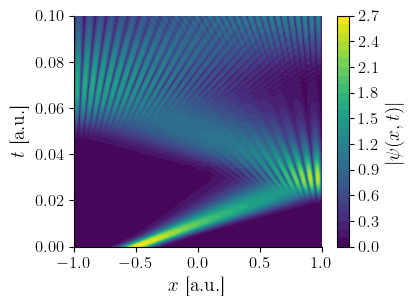
\includegraphics[width=0.6\linewidth]{figures/i_normpsi.png}
    \caption{Square root of the probability density of particle over space and time.}
    \label{fig:i_normpsi}
\end{figure}

\paragraph{Position and momentum} Now that we've seen the general "motion" of the particle, let's analyse some of its properties. Firstly, its average position is shown in \autoref{fig:i_xmoy}. We can see it initially moves as we would expect a classical particle to move (which we will compare later). When it reaches the right hand side border, it gets reflected and the average position seems to move a bit slower than before the reflection, before regaining the same speed. On the second bounce however, the average position seems to stabilise a bit, which is coherent with what we saw before: the reflections seperate the wave function in multiple thinner parts. The average position then doesn't mean very much, with the position distribution being multiple similarly sized peaks. \autoref{fig:i_pmoy} shows the average momentum of the particle. The momentum remains constant before the particle "collides" with the wall, which is also what was observed with the constant average position change on the previous figure. After the collision, the sign of the momentum flips around, meaning the wave is moving left. It is not an abrupt change, as would be expected from a wave. After a second reflection, the average momentum doesn't seem to reach the initial momentum again. This could be explained because of the spreading of the wave, where on average the wave moves slower than initially.

\begin{figure}[h]
    \centering
    \begin{subfigure}{0.48\linewidth}
        \centering
        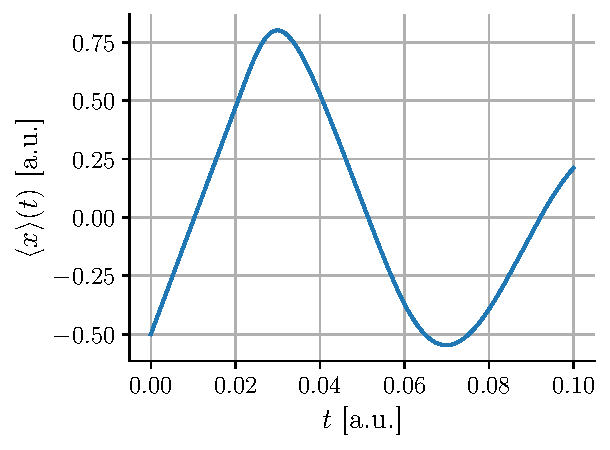
\includegraphics[width=\linewidth]{figures/i_xmoy.pdf}
        \caption{Average position}
        \label{fig:i_xmoy}
    \end{subfigure}
    \begin{subfigure}{0.48\linewidth}
        \centering
        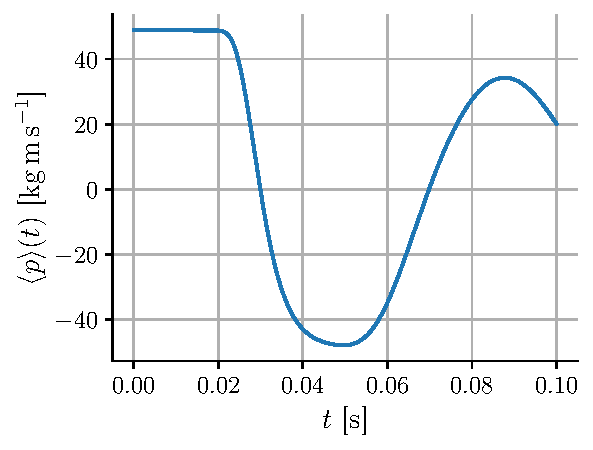
\includegraphics[width=\linewidth]{figures/i_pmoy.pdf}
        \caption{Average momentum}
        \label{fig:i_pmoy}
    \end{subfigure}
    \caption{Average position and momentum of a quantum particle in an infinite potential well}
    \label{fig:i_xmoy_pmoy}
\end{figure}

\paragraph{Uncertainty} For a quantum particle the uncertainty of its position and momentum is also a key property. \autoref{fig:i_deltax} shows the increasing uncertainty in position. It increases almost constantly, only decreasing when the wave change direction. This behavior is expected, considering we don't measure its position during the simulation. On the momentum side, \autoref{fig:i_deltap} shows the uncertainty in momentum. As opposed to the position spread, the uncertainty in momentum increases sharply at the times when the wave is reflected, increasing from less than 10 a.u. to about 50 a.u., before decreasing again to about 10 a.u.. Every reflection increases the spread of momentum on average. This will be further commented on when looking at the Heisenberg uncertainty principle.

\begin{figure}[h]
    \centering
    \begin{subfigure}{0.48\linewidth}
        \centering
        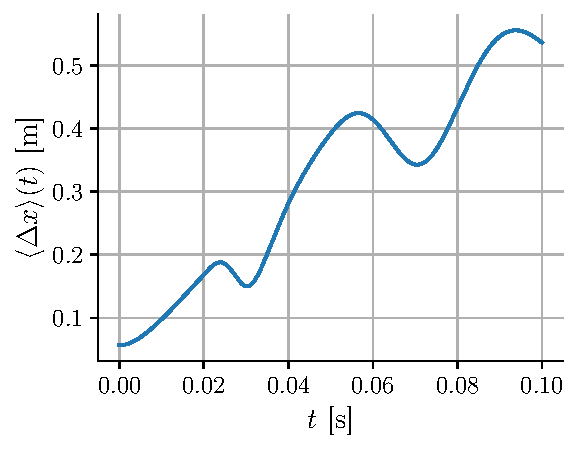
\includegraphics[width=\linewidth]{figures/i_deltax.pdf}
        \caption{Position spread}
        \label{fig:i_deltax}
    \end{subfigure}
    \begin{subfigure}{0.48\linewidth}
        \centering
        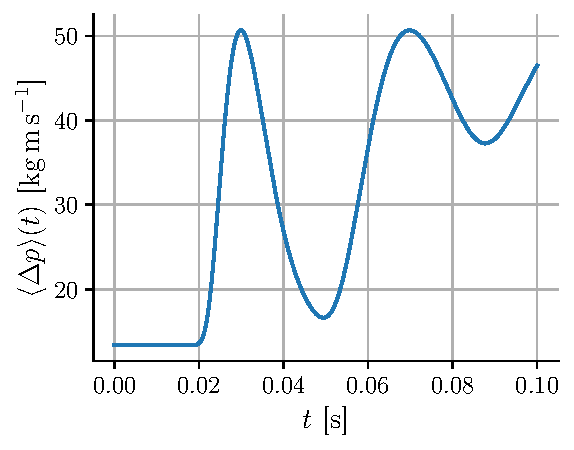
\includegraphics[width=\linewidth]{figures/i_deltap.pdf}
        \caption{Momentum spread}
        \label{fig:i_deltap}
    \end{subfigure}
    \caption{Spread over time of the position and momentum of a quantum particle in an infinite potential well}
    \label{fig:i_deltax_deltap}
\end{figure}

\paragraph{Group and phase velocity} Looking at the real part of the wave in \autoref{fig:i_repsi} allows us to notice a difference between the phase and group velocity. Indeed, we notice that peaks of the real part move along a slightly different path than the probability density shown before, meaning that the phase velocity is different to the group velocity: the wave disperses. The phase velocity can be read with the slope of the peaks of the real part, using \(\dd x / \dd t = v\). From this we see that phase velocity is slower than the group velocity, as the slope \(\dd x / \dd t\) of the peak of the probability density is greater than that of the real part. The waves with slightly different initial velocities also split appart, resulting in the effect seen in \autoref{fig:i_normpsi} before. The speed of the peaks of the real part of the wave also decrease when approaching the walls, as can be seen by the slight curvature of the peak lines.
\begin{figure}[h]
    \centering
    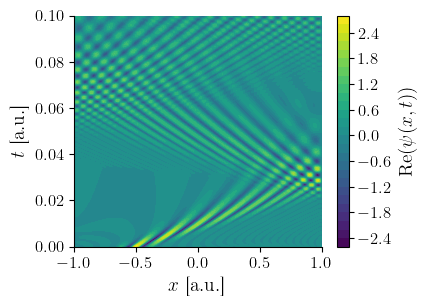
\includegraphics[width=0.6\linewidth]{figures/i_repsi.png}
    \caption{Real part of the wave function of a quantum particle in an infinite potential well}
    \label{fig:i_repsi}
\end{figure}

\subsubsection{Comparing with classical particle}

It is also interesting to compare a quantum particle with a classical particle sharing some physical properties. First looking at a particle starting with the same initial energy as the quantum particle, i.e. staring with a speed \(v\) such that:
\begin{equation}
    E = \frac{p^2}{2m} \stackrel{m=1,\ p=mv}{\implies} v = \pm \sqrt{2E}
\end{equation}
we obtain the movement shown in \autoref{fig:i_classical_vs_quantum_energy}. We chose the positive solution as we want both particles to move in the same direction initially. The same was done for a particle sharing the same initial momentum as the quantum particle, shown in \autoref{fig:i_classical_vs_quantum_momentum}. We notice that the particle sharing the same energy moves faster than the particle sharing the same initial momentum. The faster particle also doesn't match the quantum particle's average position, even before the first bounce, while the slower one matches the average position exactly, except at the borders. An interesting thing to note is that the classical particle with same momentum intersects with the average position of the quantum particle exactly at \(x=0\). From these observations we can deduce that there must be another component than the momentum contributing to the energy of the quantum particle, which is not the potential because it was set to 0.

\begin{figure}[h]
    \centering
    \begin{subfigure}{0.48\linewidth}
        \centering
        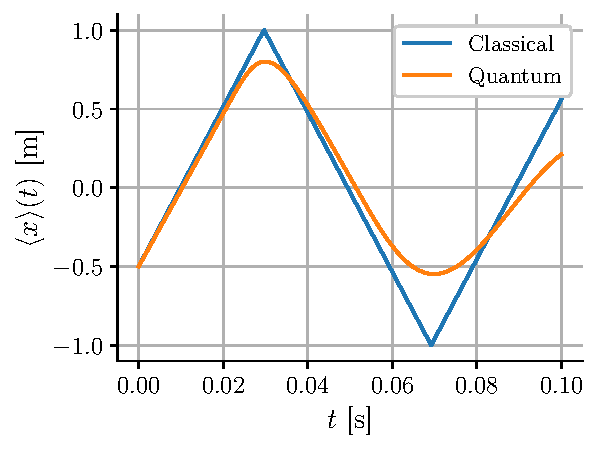
\includegraphics[width=\linewidth]{figures/i_classical_vs_quantum_energy.pdf}
        \caption{Same energy}
        \label{fig:i_classical_vs_quantum_energy}
    \end{subfigure}
    \begin{subfigure}{0.48\linewidth}
        \centering
        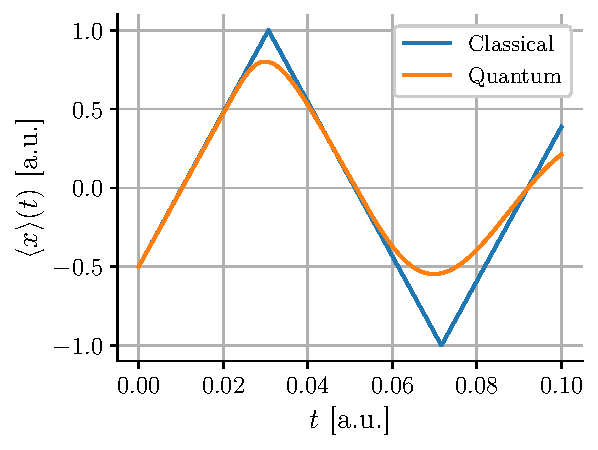
\includegraphics[width=\linewidth]{figures/i_classical_vs_quantum_momentum.pdf}
        \caption{Same initial momentum}
        \label{fig:i_classical_vs_quantum_momentum}
    \end{subfigure}
    \caption{Comparing the quantum particle to a classical particle sharing some physical properties}
    \label{fig:i_classical_vs_quantum}
\end{figure}

\subsubsection{Verifying properties of the Crank-Nicolson method}
\label{sec:crank}

Let's also verify features of the the Crank Nicolson method. Firstly, it was shown in the book \cite{physnumbook} that this method conserves energy to machine precision. This phenomenon can clearly be seen in \autoref{fig:i_conservation_energy}, with the stairs clearly showing errors due to floating point approximations. The error on energy conservation was found to be on the order of \(10^{-10}\). This method is also supposed to conserve normalisation (probability), which is shown in \autoref{fig:i_conservation_probability}. It is clear that the total probability remains constant, at \(1\). Due to the smaller values of probability, the error on conservation of probability was found to be on the order of \(10^{-13}\), smaller than the error on energy conservation.

\begin{figure}[h]
    \centering
    \begin{subfigure}{0.55\linewidth}
        \centering
        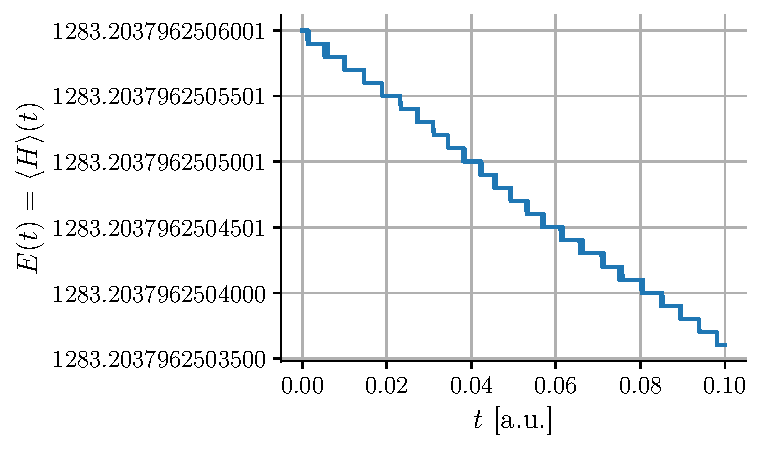
\includegraphics[width=\linewidth]{figures/i_conservation_energy.pdf}
        \caption{Energy of particle}
        \label{fig:i_conservation_energy}
    \end{subfigure}
    \begin{subfigure}{0.44\linewidth}
        \centering
        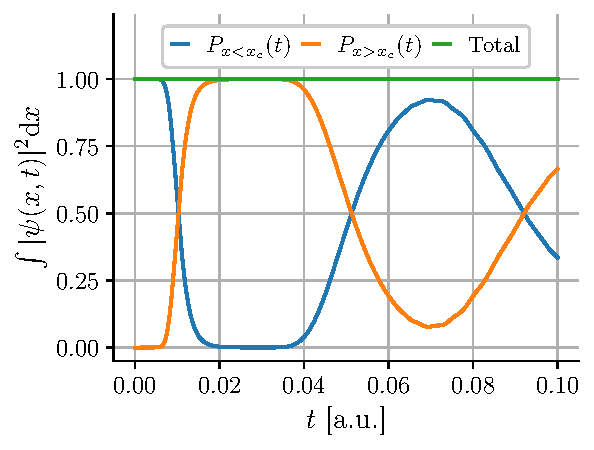
\includegraphics[width=\linewidth]{figures/i_conservation_probability.pdf}
        \caption{Normalisation}
        \label{fig:i_conservation_probability}
    \end{subfigure}
    \caption{Conservation of the particle's physical properties}
    \label{fig:i_conservation}
\end{figure}

\paragraph{Heisenberg uncertainty principle} Finally, we want to verify that the simulation produces sane physical results, more specifically that it follows the Heisenberg uncertainty principle. With our unit normalisation, this corresponds to:
\begin{equation}
    \langle \Delta x \rangle \langle \Delta p \rangle \ge \frac{1}{2}
\end{equation}
The results from the simulation are shown in \autoref{fig:i_heisenberg}. The minimal value for the product \(\langle \Delta x \rangle \langle \Delta p \rangle\) is around \(0.75\). We conclude that the Heisenberg uncertainty principle is respected. We notice that the product increases over time, meaning that we know less and less where the particle is and what momentum it has, as was seen previously.
\begin{figure}[H]
    % \vspace*{-0.5cm}
    \centering
    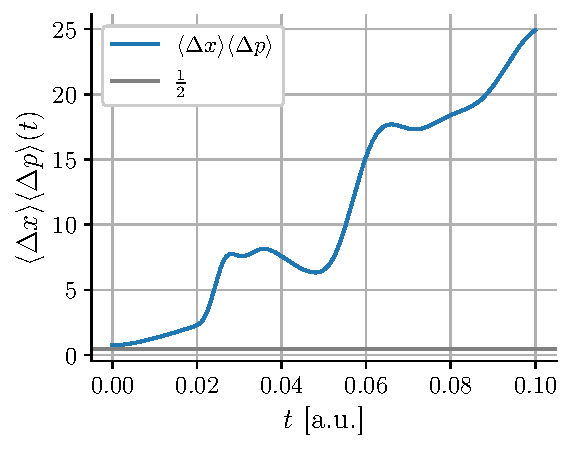
\includegraphics[width=0.45\linewidth]{figures/i_heisenberg.pdf}
    \caption{Verification of Heisenberg's uncertainty principle}
    \label{fig:i_heisenberg}
    % \vspace*{-0.5cm}
\end{figure}

% \newpage
\begin{wrapfigure}{R}{0.45\linewidth}
    % \vspace*{-0.5cm}
    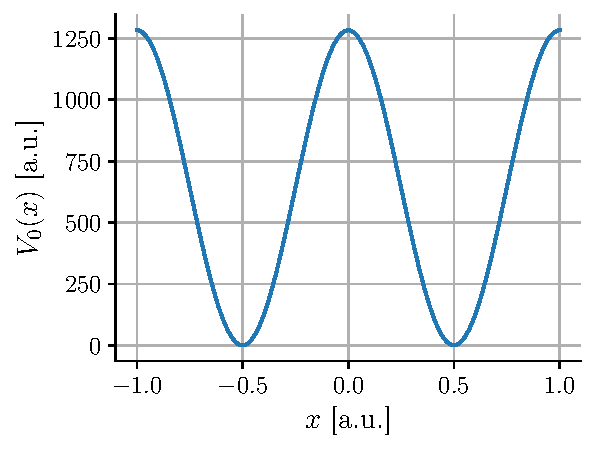
\includegraphics[width=\linewidth]{figures/potential.pdf}
    \caption{Double potential well with \mbox{$V_0 = E_\mathrm{free}$}}
    \label{fig:potential}
    \vspace*{-1cm}
\end{wrapfigure}
\subsection{Double potential well with quantum tunneling}
We now want to simulate a similar simulation with $V_0 \neq 0$. This simulation is done to analyse the quantum tunneling phenomenon that shows particles going through potential walls of higher value than their energy. For this we take various simulations with $V_0$ scaled to the energy of a free particle in an infinite potential well as determined in \autoref{sec:crank} with \autoref{fig:i_conservation_energy}: $E_\mathrm{free} \approx 1283.2$. One example of a potential with $V_0 = E_\mathrm{free}$ is shown in \autoref{fig:potential}.

\subsubsection{General behaviour of quantum tunneling}
The first analysis done is of the value $|\psi(x,t)|$ in three specific situations $V_0<\langle E \rangle$, $V_0\approx\langle E \rangle$ and $V_0>\langle E \rangle$ by taking values for $V_0$ of $E_\mathrm{free}/2$, $E_\mathrm{free}$ and $1.5 E_\mathrm{free}$ we obtain the norms of wave functions shown in \autoref{fig:tunnel_normpsi}
\begin{figure}[h]
    \centering
    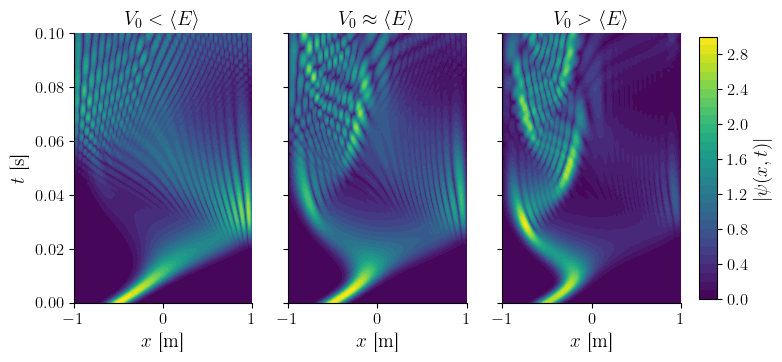
\includegraphics[width = \linewidth]{figures/tunnel_normpsi.png}
    \caption{Norm of wave functions $\psi$ for three scalings of $V_0$ relative to $\qavg{E}$}
    \label{fig:tunnel_normpsi}
\end{figure}

The results of \autoref{fig:tunnel_normpsi} show that the higher the potential $V_0$ is, relative to the average energy $\qavg{E}$, the lower the probability is of going through the maximum of the potential at $x=0$. The situation with $V_0 > \qavg{E}$ shows a very small part of the wave passing through to positive values of $x$. There is still a part so it does show that it is possible to detect the particle on the other side of a potential wall that would be high to pass in a classical description. We can quantify this by considering the probability of finding the particle on each side of $x=0$ noted as $P_{x<0}(t)$ and $P_{x>0}(t)$. This is shown in \autoref{fig:tunnel_probtrans}.
\begin{figure}[h]
    \centering
    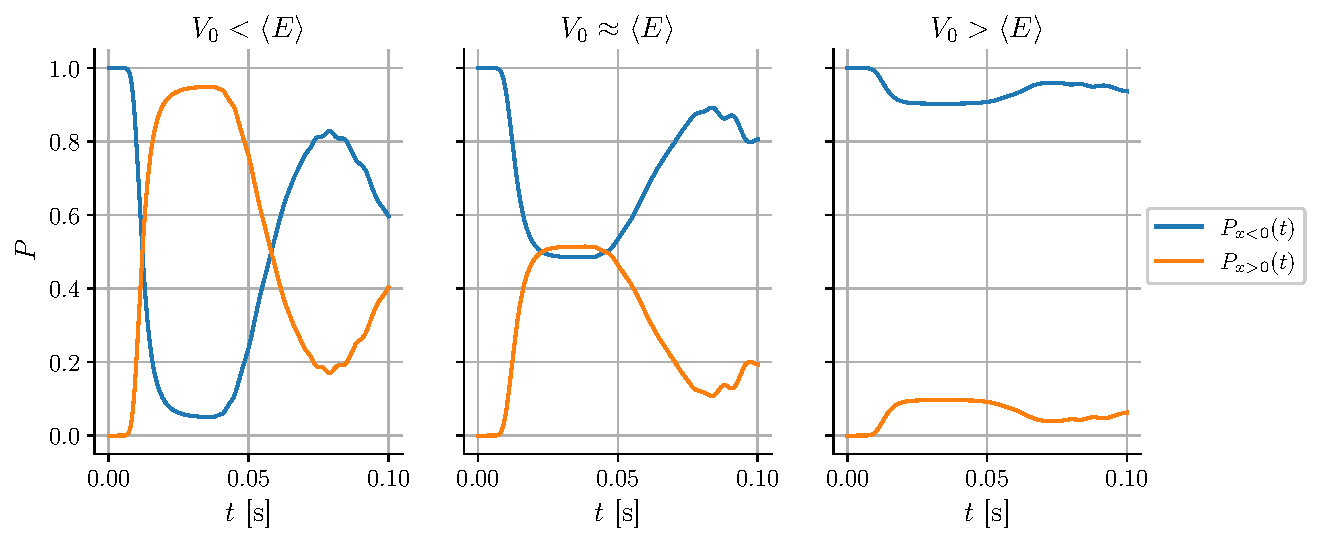
\includegraphics[width=\linewidth]{figures/tunnel_probtrans.pdf}
    \caption{Probability of transmission through the peak of a potential wall for three scalings of $V_0$ relative to $\qavg{E}$}
    \label{fig:tunnel_probtrans}
\end{figure}

Both \autoref{fig:tunnel_normpsi} and \autoref{fig:tunnel_probtrans} both show the same behavior that for $V_0<\qavg{E}$ the particle mostly goes back and forth similar to a classical particle in a potential of the shape of \autoref{fig:potential}. It is not exactly the same as a classical particle since a small probability remains on both sides at any time, corresponding to a part of the wave begin reflected, whereas a classical particle would just be on one side or the other in a deterministic way. For $V_0 \approx \qavg{E}$ we find that the probability is after the first passage almost equal around 0.5 on both sides. We can compare this to a classical system being on the unstable peak of the potential and having equal odds of falling on both sides even if the quantum behaviour is significantly different than simply falling on one side. Finally for $V_0>\qavg{E}$ we have a probability of staying left that remains close to 1 but we do see a small probability to appear on the right side. This would be impossible in a classical description and is known as quantum tunneling.

\subsubsection{Convergence analyses}
We have observed the behaviour of quantum tunneling but it can now be interesting to find the characteristics of our numerical method in the simulation of this phenomenon. For this two convergence analyses were conducted for the probability of transmission, defined as the probability to find the particle in positive $x$ at $t=0.03$ i.e. $P_\mathrm{trans} = P_{x>0}(t=0.03)$, in the case $V_0 = E_\mathrm{free}$. The first analysis was done by taking powers of 2 for the number of intervals in order to avoid side effects by taking different points for the mesh. Taking only powers of 2 guarantee that all the previous points will be the same and only points will be added in between. Another convergence in values of $\Delta t$ was also conducted. Since the moment considered is at $t=0.03$ values of $\Delta t$ adding theoretically to 0.03 were taken. This gave the two convergence in order 2 shown respectively in \autoref{fig:conv-dx} and \autoref{fig:conv-dt}.
\begin{figure}[h]
    \centering
    \begin{subfigure}{0.48\linewidth}
        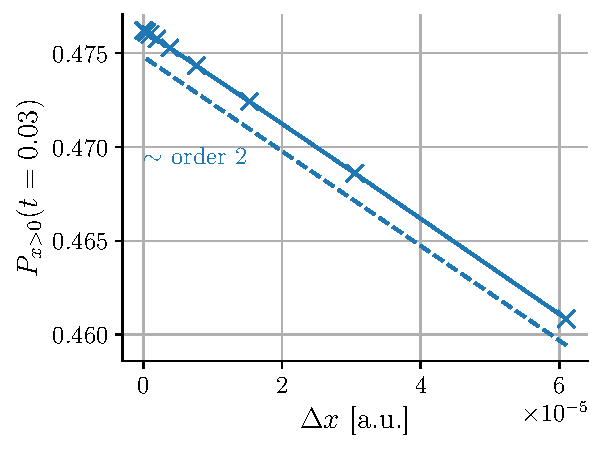
\includegraphics[width=\linewidth]{figures/conv_dx.pdf}
        \caption{}
        \label{fig:conv-dx}
    \end{subfigure}
    \begin{subfigure}{0.48\linewidth}
        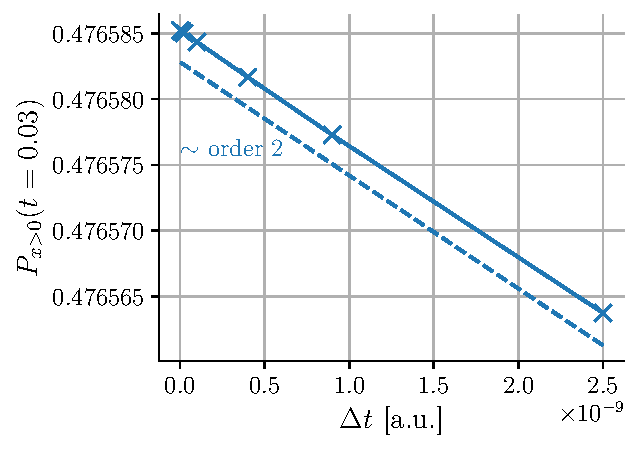
\includegraphics[width=\linewidth]{figures/conv_dt.pdf}
        \caption{}
        \label{fig:conv-dt}
    \end{subfigure}
    \caption{Convergence analysis for (a) various numbers of intervals $N$, with $\Delta x = L/N$, and (b) various timesteps $\Delta t$}
    \label{fig:convs}
\end{figure}

The converged values were also determined through a linear fit for the probability of transmission. This yielded for the convergence in $\Delta x$, $P_\mathrm{trans} = 0.476$, and for the one in $\Delta t$, $P_\mathrm{trans} = 0.477$. We do find similar and close to 0.5 probabilities as we expected. Thus we can assume that a particle arriving with an energy exactly equal to the peak of the potential would have a probability transmission of 0.5. It is important to note here that the convergences were done with $V_0 = E_\mathrm{free}$ the energy for a free particle in a null potential so in this case $V_0 \neq \qavg{E}$ it is only approximately equal.

\subsubsection{Transmission probability}
In a similar fashion the transmission probability ($P_\mathrm{trans}$) was calculated for various simulations at different energies. The results are shown in \autoref{fig:trans_energy}.
\begin{figure}[h]
    \centering
    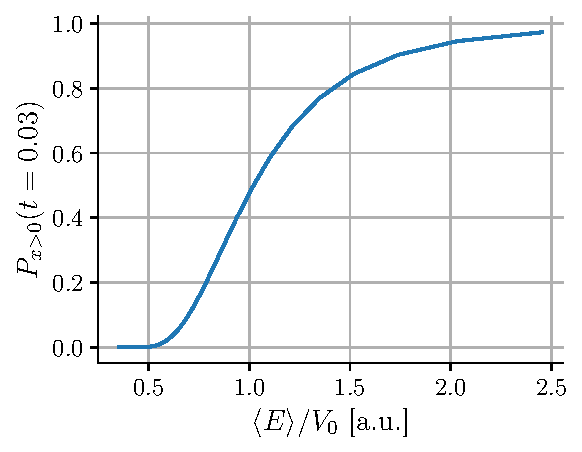
\includegraphics[width = 0.6\linewidth]{figures/energy_probtrans.pdf}
    \caption{Probability of transmission according to the ratio of the peak of potential $V_0$ and the energy of the particle $\qavg{E}$}
    \label{fig:trans_energy}
\end{figure}

The first thing we can get from \autoref{fig:trans_energy} is that as expected the value of $P_\mathrm{trans}$ when $\qavg{E} = V_0$ is 0.5. We also see that in the extreme cases $\qavg{E}/V_0 \ll 1$ and $\qavg{E}/V_0 \gg 1$ we get closer to the classical intuition with respectively the probability going to 0 and 1. This correspond to a trapped particle in the first well of \autoref{fig:potential} and to a particle with way more energy than the barrier of potential it is inside of and thus passing it easily.

\subsection{What if we changed the potential? \textcolor{white}{jk... unless?}}

Another potential was also tested to look at the behavior of a quantum particle under different conditions. In quantum mechanics a step potential is often used to simplify some problems, like with an amonia particle. Here we set the potential to be:
\begin{equation}
    V(x) = \begin{cases}
        \begin{aligned}
            &0 &&\textrm{if } x <= 0 \\
            &V_0 &&\textrm{if } x > 0
        \end{aligned}
    \end{cases}
\end{equation}
Using the same \(V_0\) as the previous section, we obtain \autoref{fig:iii_normpsi}. The behavior is very similar to a double potential well, except that we have a much more visible interference. The potential wall is also very visible in this figure, due to the reflections it causes. For a \(V_0\) close to the energy of the particle, we get an almost even split. For the case \(V_0 > \qavg{E}\), the wall acts almost like the edge, while still allowing some of the wave function through, meaning it is possible to find the particle inside the potential wall! Interference is very visible in the \(V_0 < \qavg{E}\) case, where the transmitted gets reflected back by the right hand side edge and interferes with the previously reflected wave.

\begin{figure}[h]
    \centering
    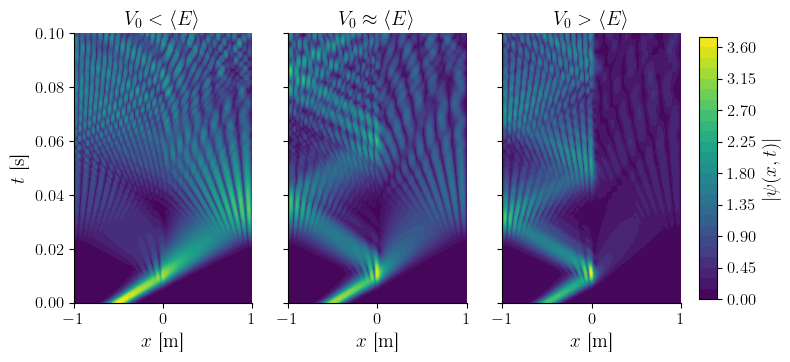
\includegraphics[width=\linewidth]{figures/iii_normpsi.png}
    \caption{Norm of wave functions $\psi$ for three scalings of $V_0$ relative to $\qavg{E}$, for a quantum particle inside a step potential}
    \label{fig:iii_normpsi}
\end{figure}

A very interesting phenomenon occurs when we consider the same potential flipped along the y axis, meaning the particle starts in a high potential area. \autoref{fig:iii_normpsi_inv} shows the obtained wave function. At the edge of the potential we notice a change in slope: the particle moves faster when in the lower potential, resulting in a refraction-like effect. The same occurs when crossing the barrier in the other direction, with the speed reducing. This is shown more clearly on \autoref{fig:iii_pmoy_inv}.

\begin{figure}[h]
    \centering
    \begin{subfigure}{0.48\linewidth}
        \centering
        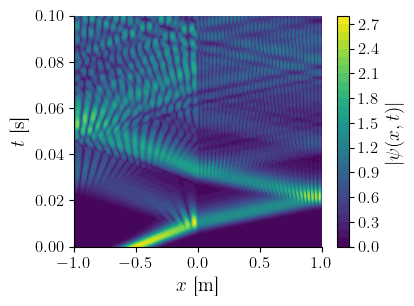
\includegraphics[width=\linewidth]{figures/iii_normpsi_inv.png}
        \caption{Norm of wave function $\psi$}
        \label{fig:iii_normpsi_inv}
    \end{subfigure}
    \begin{subfigure}{0.48\linewidth}
        \centering
        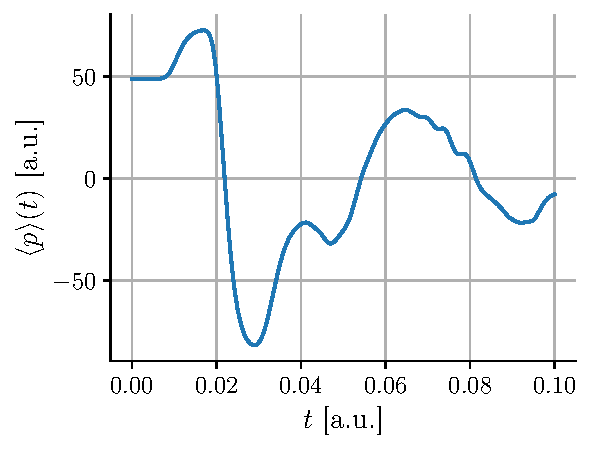
\includegraphics[width=\linewidth]{figures/iii_pmoy_inv.pdf}
        \caption{Average momentum}
        \label{fig:iii_pmoy_inv}
    \end{subfigure}
    \caption{Quantum particle starting in a high potential area, moving towards a lower potential}
\end{figure}